\documentclass{acm_proc_article-sp}

\usepackage{ascmac}

\begin{document}

\title{A Framework for Fault Tolerant Device Drivers}

\numberofauthors{1}
\author{
Hiroo Ishikawa\quad
Alexandre Courbot\quad
Tatsuo Nakajima\\
    \affaddr{Department of Computer Science, Waseda University}\\
    \affaddr{3-4-1 Okubo, Shinjuku-ku}\\
    \affaddr{Tokyo, Japan}\\
    \email{ishikawa@dcl.info.waseda.ac.jp}\\
}

\maketitle

\begin{abstract}
System software, and device drivers in particular, are particularly prone to errors, with serious consequences for the system: failures in monolithic kernels usually corrupt the whole system. This situation is particularly a problem in embedded systems where maintenance is not possible. Microkernels increased the robustness to such failures by compartmentalizing system components, but do not take their recovery into account, often leading other system components and applications that depend on the failed component to fail in turn.

In this paper, we address the problem of system components recovery in microkernel-based operating systems. In order to increase the chance of successful and transparent recovery, we propose a device driver development framework that takes recovery into account and let the driver developer specify the meaningful state of the driver, as well as the recovery policy. Giving such control to the device driver developer allows us to significantly improve recovery of failed drivers, by erasing and reconstructing meaningless driver state and reprocessing the failed request in order to keep the failure transparent to the rest of the system.

\end{abstract}

\category{D.4.5}{Operating systems}{Reliability}
\terms{Design, Reliability}
%\keywords{}

\section{Introduction}

Because of their ubiquitous and autonomous nature, embedded systems have high requirements on reliability and customizability. Appliances like mobile phones and consumer electronics experience difficulty in satisfying those requirements because they get closer and closer to desktop computers as hardware evolves.  As embedded systems and their networks increasingly support our activities and lives~\cite{Lee2006}, their reliability becomes crucial in order to compensate for their lack of system administrators.

Current embedded operating systems lack support for the reliability of device drivers.  Prior research isolated device drivers from the other parts of the operating system~\cite{Herder2007,Swift2003} and handled recovery by restarting the failed driver, but this is not sufficient for all classes of drivers.  Some device drivers hold important state to preserve over failure recovery,  including the current state of the hardware and  state that is used across requests to the driver.  Many drivers (e.g. video, audio, webcam) change the hardware state and then wait for further requests to work with the new state of the hardware.  For such drivers, a complete reset of the managed hardware is unacceptable, because (1) it would have a visible side-effect for the user or other system components that would break the transparency rule, and (2) future requests, which are tailored for the pre-failure state of the hardware, may lead to unexpected result on the reinitialized state.

We built a framework for resilient device drivers that is aiming at solving this problem by requiring the driver to define its recovery procedure.  Since it is difficult to discriminate data that is relevant to the driver's state from neglectable data, we decided to let the programmer choose which data of the driver must be preserved across failures, using specific compiler attributes.

The framework provides persistent memory, so that not only stateless drivers, but also drivers with state such as video drivers are able to efficiently recover in a consistent and transparent manner.  The base rule of this recovery mechanism is to only preserve what is strictly necessary to come back to the pre-failure state, and to recompute other data. That way, we can hope the cause of the failure has been wiped away.

Since our framework is based on the microkernel architecture, device drivers written with it run in user mode, and are isolated by a protection domain for fault containment.  Microkernel architecture contributes to our requirements because system components are isolated into protection domains, encouraging better decomposition of system services.  We adopt L4 microkernel as our kernel, a commonly-used solution in contemporary embedded systems~\cite{Heiser2007}.

We conducted several case studies to show the feasibility and efficiency of our device driver framework. For example, we were able to completely and transparently recover on a character device driver (parallel port driver) without losing or duplicating data. In addition, we were also able to recover from a video driver without affecting client applications.  A fault injection tests shown that the down time of the device driver is approximately 2 ms.

The remainder of this paper is organized as follows.  The next section describes prior research projects on the reliability of device drivers.  Section~\ref{s:design} describes ArcOS, the operating system used to implement our work, and the idea of our framework.  Section~\ref{s:impl} details the implementation of the framework.  Section~\ref{s:eval} evaluates the framework in terms of reliability and overhead, and section~\ref{s:sum} concludes the paper.


\section{Related Work}
\label{s:rel}

Device drivers are just a class (although very specific) of software. Therefore, this section deals with both research work dedicated to the recovery of device drivers, but also to research designed for general software but which ideas can be applied to device drivers.

Lowell et al. \cite{Lowell2000} made a classification of software failures. They distinguish between \emph{stop failures} (i.e. a program stopped because of an external reason, such as a \emph{kill} signal or a power outage) and \emph{propagation failures} (the program stopped because of an internal bug that drove it into a unacceptable state). Stop failures are easy to recover, as the program has been interrupted during its regular operation. Therefore, provided an earlier snapshot of the running program is available, it is usually enough to restore it and continue the execution of the program, that will this time pass the failure time successfully if the external factor that stopped it previously is not repeated again.

More challenging are propagation failures. These failures are caused by a transient bug\footnote{A transient bug or Heisen-bug is a bug that only appears occasionally and is not easily repeatable~\cite{Gray1985}.} into the running program, that lead it to failure. The time of failure and time of bug are usually different --- and can be very distant. Moreover, figuring out when the bug entered the program at the time of failure is extremely difficult. As a consequence, restoring the program to a previous state does not ensure recovery, as it is very possible that the restored state is already contaminated and will identically lead to a failure. Moreover, even if the system is restored to a state prior to the bug, nothing can ensure that the buggy conditions will not appear again during the next run.

Rx~\cite{Qin2007} tries to address this last problem by dynamically changing the execution environment based on the failure symptoms, in the hope that the change will allow the program to overtake the failure point, after which it returns to normal operation mode. Environmental changes include allocate more memory than initially asked to prevent buffers overrun, avoiding to recycle free buffers, and so on.

These recovery techniques allow to successfully recover a non-neglectable part of failure conditions. We want to address the recovery of device drivers, one class of software which is particularly exposed to transient bugs~\cite{Chou2001}, and for which failure can have very severe consequences.

Up to now, recovery of device drivers has been based on restarting. For instance, Nooks~\cite{Swift2003,Swift2006} isolates device drivers from the rest of the kernel and is able to transparently restarts then upon failure. A similar feature is provided by Minix 3 with its reincarnation server~\cite{Herder2007}. These recovery mechanisms are all based on the assumption that the restarted driver has no state of its own.

This is unfortunately not the case of all device drivers. For instance, character devices usually treat data as a stream and may fail in the middle of a treatment. In this case, simply restarting the driver and reissuing the faulty call may result in duplicated work being performed.

Another state that is important to preserve during recovery is the state of the managed hardware, if any. Indeed, when run, drivers typically initialize the hardware to an ``initial state'' and wait for instructions about how to control it. Such control may put the hardware into a different state, and sudden reinitialization would then cause a disruption in the user experience. Not to mention that applications calling the driver may still rely on the driver being in the pre-crash state, and may then issue unexpected commands, possibly causing the driver or the application itself to fail again.

Our goal in this paper is to propose a framework for device drivers that takes recovery into account. It provides a general design pattern for drivers, as well as facilities to allow the driver maker to control recovery and restore the driver's state. In the next section, we will describe the framework's structure.

\section{A Framework For Recoverable Device Drivers}
\label{s:design}

In this section, we will describe the design of our framework for recoverable device drivers. It provides a simple way to write drivers that is consistent with the server philosophy of L4, and also gives the tools necessary for the programmer to consider recovery. Its recovery procedure is to restart the failed driver while preserving data that the programmer has marked as significant for recovery.

\subsection{State of Drivers Across Recovery}
\label{s:fw}

As we saw in previous section, the main issue with transient propagation failures is that they corrupt the state of the program, and will invariably lead to another failure unless the corruption is cleared. Therefore, clearing the state of the failed program (e.g. through a complete restart) is the most efficient way to recover the software.  However, this extreme solution is not acceptable in the original condition because the internal state of the software is completely lost.

Our strategy for recovery is to clear as much of the driver's state as possible, while preserving the essential state. We restart the driver completely, while preserving certain data that the programmer marked as significant for recovery.  Upon restart, the driver is branched to an alternate entry point that is responsible for restoring its state from this persistent data. Once the recovery is performed, and provided this persistent data has not been corrupted itself, the driver can reprocess the request that caused its failure.  Since we only consider the transient bugs, we can expect the reprocess doesn't generate the same error.

There are two design choices that derive from this statement:
\begin{enumerate}
\item The framework must be able to preserve data that is significant to the state of a driver. This generally includes any data that cannot be recomputed identical to the pre-failure condition.
\item Upon driver restart, the failing operation must be re-performed.
\end{enumerate}

The last requirement is easily satisfied by the design of microkernels.  In microkernels, device drivers, like any other system part, are servers that react on and reply to requests that arrive in the form of messages. If we include this design in our framework, it is easy to consider a message treatment as the atomicity of our recovery system, and to send the message that triggered the failure once the driver is recovered.

As for the first requirement, the difficulty of discriminating between significant and insignificant data is what makes recovery of propagation errors difficult. If not enough state is dropped, the corruption of the system state may survive the recovery; on the other hand, if too much state is reinitialized, complete recovery is not possible and the behavior of the recovered driver may differ from what is expected. As a recovery framework cannot decide what differentiates useful from futile state, we decided to let the programmer directly specify which of its variables should survive a recovery. In general however, the following rules apply.

\paragraph{Significant state}
The state that should be preserved is classified into the following two categories.
\begin{itemize}
\item Driver data that reflects the state of the hardware.  If a driver and managed hardware are out of sync, there is a high chance that the next commands issued by the driver will have unexpected results.
\item Internal driver state that must survive across requests. This may include state that deals with data being provided by the managed hardware. For instance, if a serial driver sends data to the serial port from a buffer at the time of failure, recovery must be aware of the position at the time of failure in order to avoid sending the same data again.
\item Communication state has to be treated in a way that communication partners can continue their operations no matter if the communication failed.
\end{itemize}

\paragraph{Non-significant state}
State that is local to the processing of a request and is not significant as long as a side-effect has not been performed by the driver. All the input data of a request is contained into the incoming message, that is replayed once the driver is restarted. Therefore, it is safe and desirable to discard any local data created during this process, as it is likely that the corruption occurred there. Our policy of restarting the driver (even though through an alternate entry point) ensures that all local state is discarded.

Before describing our framework, we will first give a brief description of the ArcOS operating system, on which it is based.

\subsection{ArcOS}
\label{s:arc}

ArcOS is a multiserver operating system built on top of the L4 microkernel (figure~\ref{fig:arc})~\cite{L4X2}.  L4 provides minimum fundamental abstractions such as threads, IPC (for \emph{inter-process communication}), and address spaces. System components such as drivers run in user mode process and each of them is isolated by protection domains that are crucial for fault containment. ArcOS currently runs on Intel IA32 architecture.  Future releases will also support the SuperH architecture, which is often used for embedded systems.

\begin{figure}[ht]
\centering
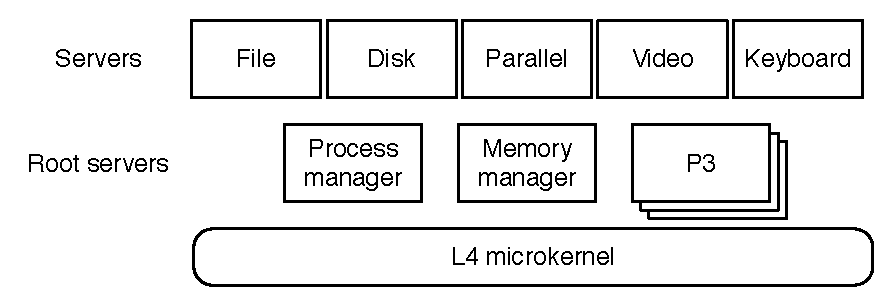
\includegraphics[scale=0.5]{figures/architecture}
\caption{The architecture of ArcOS}
\label{fig:arc}
\end{figure}

A process under ArcOS communicates with other processes via the L4 synchronous IPC mechanism.  An IPC can be either synchronous or asynchronous.  Since an IPC message payload is limited to tens of bytes, processes can use shared memory pages to exchange a large amount of data. The IPC state of a process, as well as memory page faults, are handled by its pager, a dedicated process called P3 (for \emph{Per-Process Pager}, see figure~\ref{fig:p3}). The pager is also in charge for loading the program, which, as we will see, confers it a crucial role in recovery.

\begin{figure}[ht]
\centering
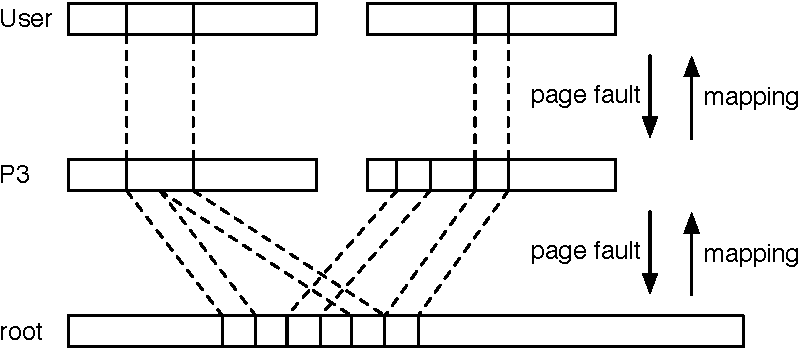
\includegraphics[scale=0.5]{figures/p3}
\caption{The relationship between the root pager, per-process pagers and user processes}
\label{fig:p3}
\end{figure}

This particular design, in which P3 acts as a ``nurse'' for the process it manages, further increases the isolation of processes and influences how our recovery mechanism will perform.

\subsection{Driver Framework Design}
\label{sec:design-framework}
Just like any other process, a device driver is loaded and started by its own instance of P3. This particularity will greatly influence the design of our driver framework. First, the task of putting the driver back into recoverable operation is left to P3. Also, the driver can have different entry points, depending on whether it is being recovered or not. Indeed, we consider that there are four main states in the life of a device driver:
%The goal of the framework is to provide some rules for definining the way of recovery and persistent data to a developer.  The device driver under the framework implements the following four functions.

\begin{description}
\item[Initialization.]
Where the device driver initializes managed peripherals and its internal data structures. This state is only entered once, when the driver is started.

\item[Service loop.]
In ArcOS, a device driver is a server process, which waits for requests from its clients: for instance, a file system server is a client of a disk driver. The service loop implements that request handling mechanism, by associating messages to handler methods.%  The framework's recovery policy assumes that the service loop crashes.

\item[Finalization.]
In case of normal termination of the driver, it may be necessary to perform finalization tasks like synchronizing the hardware state to the current driver state, or safely terminating the current sessions with its clients.

\item[Recovery.]
Every device driver is supposed to implement its crash recovery procedure. Should a failure occur within the driver, the framework restarts it and invokes this function instead of the initialization function. It is then up to the recovery function to ensure the driver is put back into a state where it can perform again, by using the recovery mechanisms provided by the framework.% While its stack, heap and registers are initialized, the persistent memory area state is preserved to its pre-failure state.
\end{description}

On initial start, the initialization function is called, followed by the service loop and (provided the service loop ever exits or the driver is unloaded) the finalization function. Should a failure occur while the driver is processing a service request, the non-persistent part of its address space is reinitialized and the driver is reloaded, entering this time the recovery function before pursuing on the service loop again (figure~\ref{fig:driverstatemachine}).

\begin{figure}[ht]
\centering
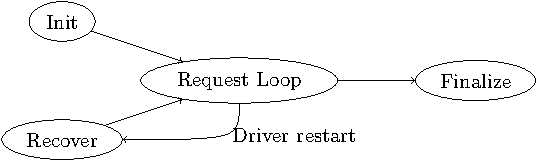
\includegraphics[scale=0.6]{figures/driverstatemachine}
\caption{States of a device driver.}
\label{fig:driverstatemachine}
\end{figure}

%While the initialization is invoked in normal mode, the recovery is invoked when the driver failed.  The main and the finalization are common in either normal or recovery mode.  In either case, the address space of a device driver is initialized; the program code is loaded from a disk, its heap and stack areas are initialized, and the CPU registers except the instruction pointer are reset. On the other hand, the driver keeps its process number (used by client applications to communicate with it), and the persistent memory area is preserved.

%The framework and a device driver forms a single process (Figure~\ref{fig:fw}).  The runtime of the framework processes communications with clients and invoking handlers defined by the driver implementation.
The framework is designed as a wrapper around the actual driver that provides this basic shape as well as other facilities for recovery (figure~\ref{fig:fw}). Using it, the driver writer only has to write behaviors for the initialization, finalization and recovery functions, define the protocol used by the driver to communicate with client process, and associate function handlers to the different kinds of messages the driver can handle. All message and error handling is then performed by the framework on this basis.

\begin{figure}[ht]
\centering
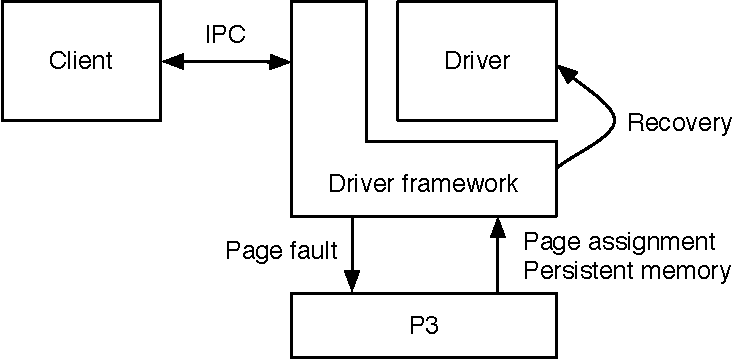
\includegraphics[scale=0.6]{figures/framework}
\caption{The device driver framework}
\label{fig:fw}
\end{figure}

All memory management and failure detection are performed by P3 which, as the driver's pager, is immediately notified of page faults and other error conditions. Should P3 detect an invalid sequence in the driver (such as a page fault to an unauthorized address, or a division by zero), P3 will immediately stop the driver and restart it from the recovery entry point. During the driver restart process, all its address space is cleaned and reset to its initial state, with the exception of the persistent memory area which is the only state of the driver that survives failures.
% The framework relies on P3 for failure detection, persistent memory and driver restart.  The recovery sequence -- from failure detection to driver restart -- is done by P3.  There is no interactions with the framework in this sequence.

\subsubsection{Persistent memory}

When the driver fails and is restarted by P3, it tries to recover to a state that is consistent with the state of the hardware being managed and the functional state of the driver, so that the crash and recovery are completely transparent to other processes. Restoring the pre-crash state requires that data relevant to this state survives the crash. To this end, the framework provides a persistent memory area for every driver.  This area is mapped to a specific region in the address space that holds data across process restart - but do not survive normal termination of the program.  Unlike a file system, the data in the persistent memory area is stored in the original structure so that a program deals with the data as in the same way as the data segment.

The programmer is provided with a specific keyword that can be appended to variable declarations and results in these variables ending into the persistent memory area. Such declared variables remain untouched by the recovery process, and remain accessible via their pre-crash address as soon as the driver is restarted.

It is the responsibility of the driver writer to mark data that is relevant to recovery as persistent. On the other hand, the set of persistent data should be as small as possible to reduce the risk of contaminating the persistent area with a propagation fault, which would result in the same crash. The policy that we used during our own drivers development and that we found efficient in limiting the persistent memory area to the minimum is to first write the driver without recovery in mind, and then make the slight adaptations that are needed to use our recovery framework. That way, variables that end in persistent memory are well-thought and chosen accordingly to the final design of the driver. We will discuss this point furthermore in the implementation and experiments sections.

When the driver successfully recovered from its crash, it enters the service loop and immediately tries to process the failed request again.

\subsubsection{IPC continuation and disruption}
% Assuming single-threaded
A device driver has an IPC state as every communicating process does.  Across restart, the state of IPC is always preserved.  However, if the driver crashed before replying to the client (which is what happens unless the bug resides within the framework itself), leaving IPC state may block the client that is waiting for the reply from the driver.  To solve this problem, the framework always commit the last message it received into the persistent memory area.  In case of recovery, the last message is loaded from the persistent area, and reprocessed. That way, outside processes do not notice any interruption of service.

It shall be noted that the processing of the failed request may differ in case of recovery. Indeed, requests that ask a character device driver to write or read more than one unit of data from the device may rely on a buffer and an iterator. In this case, replaying the whole request from start may result in data being written multiple times or previously read data being erased. In such a case, the handler function will need to place both the buffer and the iterator into persistent memory, and notice that the handled request is a replay of a failed previous one. This is made possible thanks to a global status variable that is set by the framework when processing a failed request.

%The IPC state is discarded if the driver is restarted from scratch.  This is the case if the number of retry is failed.  For example, some kind of errors such as an error in the persistent memory causes unrecoverable failure.

%The notification is sent as a reply to the request.  However, a process may not know the failure at the time it occurs.  This may be a problem if the process identifier is refreshed.

%\subsubsection{Session}
% what if sessions are created into persistent memory? Don't they survive the crash? In that case, maybe this part is not needed.

%Processes under ArcOS share some physical pages, called {\it session}, to exchange a large amount of data with other processes.  Since some types of device driver that deal with such data often create sessions, we need to handle the state of the sessions across failure recovery.

\subsubsection{Recovery policy}

% Recovery with persistent memory
Our recovery method is based on restart recovery.  If a driver fails, the framework restarts the driver to remove the cause of the failure.  The framework first tries recovery of the driver with the persistent memory where its significant state is saved.  If the same failure still occurs over the limit time of recovery, the framework tries complete restart which discards the contents of the persistent memory in addition to the non-significant state.

% Recovery with notification
% What for? Isn't that out of scope here?
%The framework sends a restart notification to each server that has communicated with the crashed driver.  Processes under ArcOS establish sessions to communicate with others.  The framework records the active sessions.  The notification is sent in the order of connection establishment.

\section{Implementation}
\label{s:impl}

In accordance with ArcOS philosophy, both the framework and device drivers are implemented in C++.  By means of inheritance, the framework enforces device drivers to implement the recovery operations.  The runtime of the framework implements common operations such as server main loop and the definition of recovery operation flow.  The persistent memory is implemented only with the main memory to make it light-weight.

We use L4::Pistachio~\cite{L4X2} with experimental features to allow a pager to be able to control the registers and IPC state of a user process.  This feature is necessary for P3 to recover a driver.

\subsection{Driver framework}

The framework provides the \texttt{DeviceDriver} base class that enforce all device drivers to provide the mandatory operations we described in section~\ref{sec:design-framework}. Figure~\ref{fig:devicedriverclass} shows a simplified version of the declaration of this class.

\begin{figure}[ht]
\centering
\begin{screen}
\begin{verbatim}
class DeviceDriver {
protected:
  virtual status_t Service(
      const L4_ThreadId_t& tid,
      const L4_Msg_t& msg,
      L4_Msg_t& retMsg) = 0;

public:
  virtual status_t Initialize() = 0;
  virtual status_t Exit() = 0;
  virtual status_t Recover();

  status_t MainLoop();
};
\end{verbatim}
\end{screen}
\caption{A simplified version of the DeviceDriver class declaration.}
\label{fig:devicedriverclass}
\end{figure}

The \texttt{Initialize} and \texttt{Exit} methods are abstract virtual, which enforces the driver developer to implement them. \texttt{Recover} is virtual but the framework provides a default implementation that just returns an error message to P3, stating that the driver cannot be recovered. That way, it is possible and easy to write device drivers without taking the recovery aspect into account.

The other public function, \texttt{MainLoop}, is already implemented and is called by P3 after the driver is started or recovered by \texttt{Initialize} or \texttt{Recover}. It waits for incoming messages, and pass them to the \texttt{Service} method along with the identifier of the sender. It will also replay the failed request in case it notices the driver has been recovered.

The \texttt{Service} method, although declared as abstract virtual, is not to be implemented directly by the driver's writer, contrary to the other methods. Indeed, this method should mainly consist of a \texttt{switch} statement that checks the label of the incoming message, call the corresponding handler, and puts the message to return to the client into \texttt{retMsg}. As it must deal with error handling and is very repetitive, we wrote a set of macros that construct that method using the message/handler paradigm to associate message labels to the corresponding method handler. An example usage of these methods is given by figure~\ref{fig:connectors}.

\begin{figure}[ht]
\centering
\begin{screen}
\begin{verbatim}
BEGIN_HANDLERS(AudioDriver)
CONNECT_HANDLER(AUDIO_SET_VOLUME,SetVolume)
CONNECT_HANDLER(AUDIO_FLUSH_OUTBUFFER,Flush)
END_HANDLERS
\end{verbatim}
\end{screen}
\caption{Example usage of the message/handler macros.}
\label{fig:connectors}
\end{figure}

The message labels are just integers that define the protocol used between the client and the driver and may be build using an enumeration. Handler functions must follow the following prototype:
\begin{verbatim}
status_t HandlerFunction(const L4_Msg_t& msg,
                         L4_Msg_t& retMsg);
\end{verbatim}
They return in the message that is to be sent back to the client in \texttt{retMsg}.

This framework thus provides all the building blocks to write a device driver for ArcOS. By just being required to write the initialization and finalization methods and to connect messages to their corresponding handlers, the driver writer can concentrate on the functional aspect of the driver without having to worry about inter-process communication. Once the driver is written, he can then take care of the recovery aspect.

Making a driver recoverable requires to write the corresponding recovery method, and to mark relevant data to be persistent across failures. We will now see how this mechanism works.


\subsection{Persistent Memory}
The persistent memory area is designed to host data that are necessary for recovery and must survive a failure. Contrary to what can be expected from a persistent memory, it does not rely on external storage and simply consists of a special part of the main memory\footnote{Real persistent storage is not necessary here as the memory must only survive driver failures, not system restart}. Its features make it particularly suitable for embedded devices:
\begin{itemize}
\item Very lightweight: at runtime, no special handling is required for persistent data, which are accessed like any other data in main memory.
\item No data redundancy: persistent data is not a duplicate of existing data, but consist of actual runtime data in a special location of the address space.
\item Very easy to use on the programmer's side: a single macro to append to variable declarations is enough to have them located into persistent memory.
\end{itemize}

Implementation of this persistent memory is made through a cooperation of the compiler and linker. Indeed, the GCC compiler~\cite{GCCManual} provides support for section attributes that define in which section of an ELF~\cite{ELFSpec} file a declared variable should be located. By using this feature, we defined a C macro that can be appended to any declared variable in order to place it into a special \emph{.pdata} section.

\begin{verbatim}
#define IS_PERSISTENT \
  __attribute__ ((section(".pdata")))
\end{verbatim}

At link time, the LD linker is given a special link script that relocates all data in the \emph{.pdata} section together. When P3 loads the device driver binary, it detects this \emph{.pdata} section and automatically maps it into a dedicated area of the address space. (figure~\ref{fig:layout}).

\begin{figure}[ht]
\begin{center}
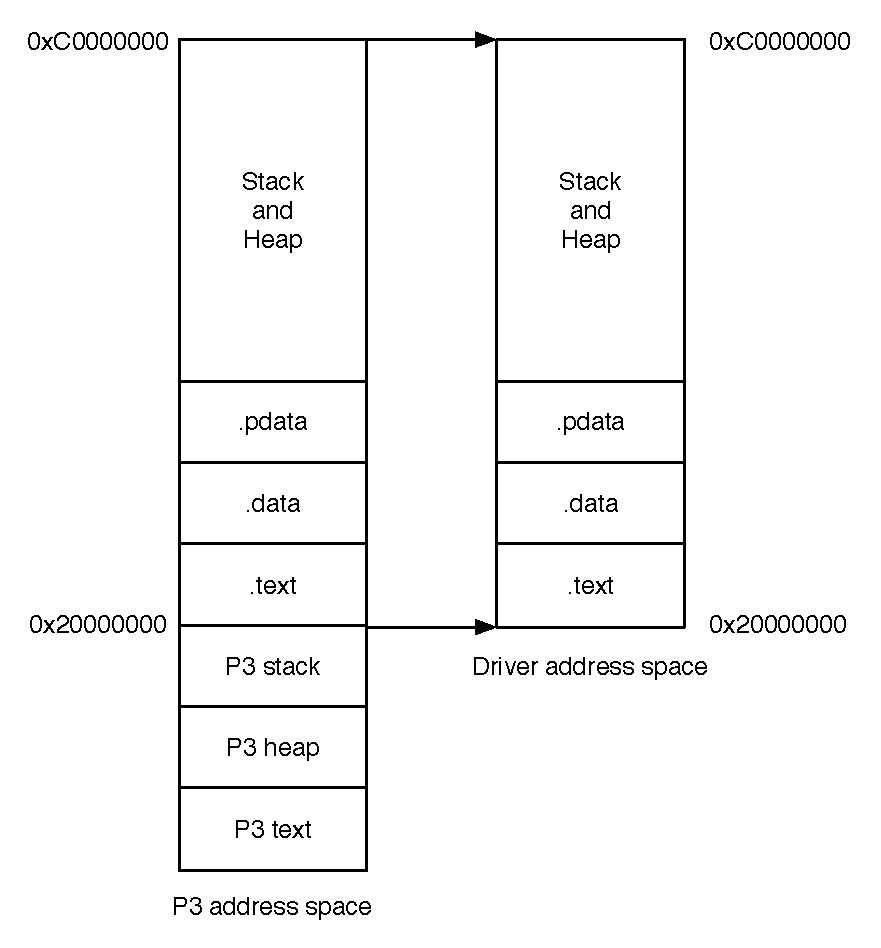
\includegraphics[scale=0.5]{figures/layout}
\caption{The memory layout of a device driver process}
\label{fig:layout}
\end{center}
\end{figure}

Each process therefore possesses its own persistent memory area. P3 assigns physical memory pages to the persistent memory area at load time, just as it does with other memory sections. However, upon a failure of the driver process, all the physical pages but the persistent memory area are unmapped. This design makes the persistent memory area absolutely free in terms of memory footprint, and virtually free in terms of performance, since only a few trivial operations must be performed by P3 at load and recovery time to support it.

We should note, however, that this memory is not transactional. It is not possible to bring it back to a previous state: this means that if the failure entered the persistent memory area, it will most likely not be recoverable.

\subsection{Failure Detection and Recovery}
Error detection is performed by the P3 instance of the device driver, because as its pager process it is in charge of handling page faults and other kinds of exceptions. Currently we only detect memory access violation.  The error detector is implemented in the page fault handler, however, it will be improved to a general error detection architecture as proposed in~\cite{Qin2007} and~\cite{Wang2006}.

The recovery process when an invalid page access (most likely due to an invalid pointer being used) is as follows: first, the faulty driver is stopped, and all its memory pages but the code and persistent data sections are unmapped. Then, the data and heap area are recreated as for when the driver is initially loaded, and an initial stack is created. P3 then invokes the \texttt{Recover} method of the driver instance, which returns a status value: it that value indicates that recovery failed, P3 then fully restarts the driver from scratch. On the other hand, if the return value indicates a success, P3 sets the global recovery flag to \emph{true} and starts the driver by invoking the \texttt{MainLoop} method in the driver's address space.

The implementation of the \texttt{MainLoop} method first checks the value of the global recovery flag. As it figures out it is set to \emph{true}, it immediately calls the \texttt{Service} method with the last message it received before the crash. Indeed, the variables handling the received message and the ID of the sender are themselves placed in persistent memory. Figure~\ref{fig:mainloop} gives a shortened version of the \emph{MainLoop} implementation, where the error handling code has been removed.

\begin{figure}[ht]
\centering
\begin{screen}
\begin{verbatim}
static L4_ThreadId_t tid IS_PERSISTENT;
static L4_Msg_t msg IS_PERSISTENT;

status_t DeviceDriver::MainLoop() {
  status_t err;
  L4_Msg_t retMsg;
  L4_MsgTag_t tag;
  if (Recovered) goto restore;
begin:
  tag = L4_Wait(&tid);
  for (;;) {
    ...
    L4_Store(tag, &msg);
restore:
    err = Service(tid, msg, retMsg);
    ...
    L4_Load(&msg);
    tag = L4_ReplyWait(tid, &tid);
    Recovered = false;
  }
  ...
\end{verbatim}
\end{screen}
\caption{Shortened version of the \texttt{MainLoop} method.}
\label{fig:mainloop}
\end{figure}

\section{Evaluation}
\label{s:eval}

In this section, we would like to evaluate the efficiency of our driver framework. The main point for a recovery mechanism is to effectively recover upon failures -- therefore, we will first illustrate how we managed to recover on two different drivers instances: first, on a character device driver (parallel port driver), a class of devices driver that are reputed particularly difficult to recover from because of the stream nature of the managed hardware. Then, we will consider recovering from a VESA video driver. This kind of driver must keep enough information about the current state of the managed hardware to ensure a complete and transparent recovery.

All our evaluations have been performed on an Intel Pentium4 3.4GHz with 1GB of main memory.  The following subsections show our case study on the framework.

\subsection{Parallel Port Driver Recovery}
Our first attempt at recovery has been performed on a very simple SPP parallel port driver. The SPP protocol is an unidirectional protocol designed to send data to a printer. Because of its simplicity, we chose to implement it in order to be able to easily demonstrate how recovery can be managed in this class of drivers.

Character devices drivers are indeed reputed to be very difficult to recover from: character devices indeed deliver or receive their data one data of unit at a time, and do not support random access. Therefore, if a data is read by the driver and lost in the failure, failure transparency is broken. All the same, if a service fails when sending data to a character device, transparent recovery implies that the same data is not sent twice. This requires that the driver keeps track of its internal state and uses it upon failure. We will show how we implemented this feature using our framework.

\subsubsection{Driver Implementation}
The parallel port driver that we implemented covers the SPP protocol~\cite{Peacock2007}. This protocol, the simplest that can be used on recent and older parallel ports, is an unidirectional protocol designed to send data to a printer. The driver accepts \texttt{WRITE} requests that embed the data to be written to the port. This task is performed by the \texttt{writeData} function, which writes an array of bytes to the parallel port and which simplified code can be seen on figure~\ref{fig:writeData}.

\begin{figure}[]
\centering
\begin{screen}
\begin{verbatim}
1 status_t writeData(const char *const buffer,
2                    size_t count) {
3   Byte control = inb(CONTROLPORT);
4 
5   for(int i = 0; i < count; i++) {
6     control &= ~STROBE;
7     outb(DATAPORT, buffer[i]);
8     outb(CONTROLPORT, control);
9     L4_Sleep(SEND_DELAY);
10    control |= STROBE;
11    outb(CONTROLPORT, control);
12    L4_Sleep(SEND_DELAY);
13    ...
14  }
15  ...
\end{verbatim}
\end{screen}
\caption{Simplified version of the \texttt{writeData} function used to write data to the parallel port.}
\label{fig:writeData}
\end{figure}

Writing a byte to the parallel port consists in setting the data port to the value of the byte to be written, and to lower the \texttt{STROBE} bit of the control port for at least 5 milliseconds so that the printer is aware that new data is written and can read it. After that, \texttt{STROBE} is set again for 5 milliseconds before the next byte is written.

When receiving a \texttt{WRITE} request, the handler just calls this function with the byte array and length of data as parameter. The rest of the driver is very simple: it has no initialization or exit function. Therefore, and providing that the driver framework is safe, failures can only happen in the \texttt{WRITE} request handler and the \texttt{writeData} function, in which case P3 will restart the server and replay the last message received. If the request has not been processed at the time of failure, then recovery is completely transparent.

If the \texttt{writeData} function was in the midst of writing data from the buffer, then data may be written twice as the whole request is being reprocessed. Therefore, in order to ensure transparent recovery, we need to instrument the \texttt{writeData} function in such a way that is does not repeat already sent data.

\subsubsection{Recovery Handling}
The parallel port driver is a typical example of driver that needs to keep some intra-request data persistent in order to achieve transparent recovery. All the input data (contained into the message) are implicitly preserved by the framework. However, the stream nature of the parallel port also requires to keep track of the amount of processed data, symbolized by the \texttt{i} variable.

This means that \texttt{i} must also be made persistent. Moreover, we have to be very careful about its update time: in the implementation of figure~\ref{fig:writeData}, \texttt{i} is only incremented at the end of the loop. If a failure occurs between the moment \texttt{STROBE} is set down (line 8) and the end of the loop, the last character would be written twice when recovery takes place. Therefore, \texttt{i} must be updated right after the character is sent to the printer. Figure~\ref{fig:writeDataRecover} gives the code of the recover-friendly version of this method.

\begin{figure}[]
\centering
\begin{screen}
\begin{verbatim}
1 static int i IS_PERSISTENT = 0;
2 status_t writeData(const char *const buffer,
3                    size_t count) {
4   Byte control = inb(CONTROLPORT);
5
6   if (!Recovered) i = 0;
7   while (i < count) {
8     control &= ~STROBE;
9     outb(DATAPORT, buffer[i]);
10    outb(CONTROLPORT, control);
11    i++;
12    L4_Sleep(SEND_DELAY);
13    control |= STROBE;
14    outb(CONTROLPORT, control);
15    L4_Sleep(SEND_DELAY);
16    ...
17  }
18  ...
\end{verbatim}
\end{screen}
\caption{Modifications made to the \texttt{writeData} function to make it recovery-friendly.}
\label{fig:writeDataRecover}
\end{figure}

The first notable thing is that the \texttt{i} iterator is declared outside of the function to survive its local scope, and is made persistent. Then, it is reset to its initial (0) value only if the IPC being processed is not the replay of a recovery. Finally, \texttt{i} is incremented as soon as \texttt{STROBE} is set down, as from this time we can guarantee that the printer will receive the byte being issued if \texttt{STROBE} remains down at least 5 milliseconds.

The recovery function of the driver is limited to ensuring this last condition: it just waits for 5 milliseconds to ensure the current state of the \texttt{STROBE} bit is acknowledged, and then sets it high so that the port is ready to send data again.

\subsubsection{Results}
We tested the two versions of the parallel port driver by randomly setting the \texttt{buffer} variable and accessing it within the \texttt{writeData} function in order to make the driver fail. As expected, the non-instrumented version re-emitted the whole buffer to the parallel port, resulting in duplicated data being sent. On the other end, the recovery-friendly version never lost data, and thus recovered completely totally transparently.

This result is very significant regarding the capability of this framework to produce reliable drivers. Previous research on device drivers and software recovery essentially relied on simple driver restarting or resuming from a previously captured snapshot. Both methods would fail to recover this driver in most cases. Restarting the driver automatically implies that the failed IPC is entirely processed again, likely resulting in duplicate data being written. Snapshotting the entire process does not ensure that the latest snapshot is recent enough to have the data iterator up-to-date with the current state of sent data. Moreover, it is also likely that the corruption of the \texttt{buffer} variable resides in the snapshot, resulting in the same failure occurring after recovery.

By letting the programmer decide which data is relevant to recovery, and by discarding all other data within the process, we ensure that important data is always preserved while maximizing chances to erase the cause of failure. This allows even very state-dependant drivers like character devices drivers to recover successfully from failures.

\subsection{VESA VBE Graphic Driver}
The VESA BIOS Extension (VBE~\cite{VBE}) specifies a standard and unified way to use graphic hardware. A program written using the VBE API can use any graphic board that supports the standard without regard for the actual underlying hardware. This standard has been widely used in the 90's and is still of use as a fallback solution for when a dedicated, optimized driver is not available for a given video board.

\subsubsection{Driver Implementation}
VBE provides APIs for getting information about the video card (total memory, supported modes and their properties, \ldots), setting a particular video mode, getting the hardware address of the video framebuffer, and controlling various other aspects of the graphic board. The driver that we implemented provides a view over the graphic board and its video modes to let the client programmer choose the desired video mode, as well as an access to the video framebuffer.

To allow this, the driver must first get all this information for itself. On initialization, the driver uses the VBE API to fill two kinds of structures: the \texttt{Screen} information (video board properties like vendor, amount of memory, \ldots) and a list of \texttt{VideoMode}, which gives information about the resolution, pixel properties, and access rules of a given video mode. In particular, every mode descriptor holds the hardware address of its framebuffer.

When the video driver has retrieved this information, it must expose it to the client. It does so by storing it all within the same memory page, and by mapping this page read-only into the client's address space. That way, the client can examine the list of available video modes, and choose a mode to use.

When the client requests a video mode to be set, the driver must perform two operations: setting the video mode to the graphic board, and mapping the framebuffer to the client so it can draw on the screen. To do this last operation, the driver makes a privileged request to obtain a mapping of the hardware address of the framebuffer, then maps it to the requesting client. It also keeps the process ID of the client in memory: as the screen is not a multiplexable resource, only one program can access it at a time. Subsequent requests to set a video mode from other programs will result in a ``Resource Busy'' error until the process that initially requested access to the screen releases it or terminates.

The video driver then holds the following information across requests:
\begin{enumerate}
\item Properties of the video board and list of supported modes (in the same memory page),
\item Current holder of the screen,
\item Current video mode,
\item A mapping of the framebuffer of the current video mode.
\end{enumerate}

On driver failure, the first information is easily retrievable by querying the VBE API again at initialization time. However, since the driver has been restarted, this would happen in another memory page, and this duplicated information will make that the mapping of the current client would not correspond to the mapping of the driver. More serious, the current holder of the screen and current video modes would be lost ; this means that the driver does not know who is the current holder of the screen, or if there is even a holder. In these conditions, if another process requests access to the screen, and the driver gives it, two processes would access the screen concurrently. Despite of the graphical glitches that would occur from this, more serious problems can appear because the second process can have set the hardware into a video mode that makes the framebuffer mapping of the first process obsolete -- in this case, paint attempts from the first process would produce unpredictable results on the hardware, which may fail in turn, and the whole system with it.

\subsubsection{Recovery Handling}
There are two problems to solve in order to make the VBE driver transparently recoverable. The first one is to ensure that holder and current mode information are preserved across failure. The second is to avoid querying again the video card for its capabilities and supported modes on recovery, in order to avoid wasting a memory page.

The first problem is easily solved by placing the variables for current holder and video mode into persistent memory. Since the framebuffer is recoverable from this information and its hardware address is fixed, we prefer to retrieve it again on recovery to comply with our ``preserve only the necessary'' policy.

The second problem requires that the memory page that holds card and modes information is also placed into persistent memory. As it is dynamically allocated by the driver at initialization time, this requires the use of a dedicated persistent memory allocator, which works the same way as a classical memory allocator (but on the persistent memory part of the address space). Being placed in a part of the address space that is not cleared on failure, the memory mapping of the card and mode information is preserved across failure and remain the same between the driver and its potential client.

Recovery is limited to restoring the mapping of the video framebuffer. We chose not to keep this mapping in persistent memory because it is easily retrievable, and in the case it is the source of the failure we prefer to request it again.

\subsubsection{Results}
Once the video mode is set and the framebuffer mapped to the client process, the video driver does not interfere with the drawing operations themselves, which are directly performed by the client by writing the video framebuffer. It may, however, be requested for tasks like changing the beginning address of the physical screen (to support double buffering) or updating the color palette. Also, another process can request access to the screen, in which case it should be denied.

We introduced a bug in this last event that makes the driver fail, ran a graphical program, and let another process try to get access to the screen at random times. As we could expect, the restoration was effective and complete, and the graphical client was not perturbed by the video driver crashing: indeed, drawing operations are not conditioned by the driver being unavailable, and the only potential delays happen when the client asks the driver the change the displayed video page while the latter is being recovered, as the IPC is delayed. However, we have not perceived any visible slowdown. The next section explains this by evaluating the performance of our recovery.

\subsection{Performance Evaluation}
We started by evaluating the overhead of P3.  P3 redirects all page mapping requests to the root pager, which holds all physical pages.  We measured the cycle count of handling a page fault and the subsequent page mapping.  The page fault handling with P3 takes approximately 1.5 times as many cycles as the one without P3.  Since page faults only occur the first time a user process accesses the page, we consider the resulting overhead as not critically harmful to performances.

Total downtime of the framework upon a failure has been measured to 0.2 ms.  To get this metric, we injected a simple fault that results in a memory access violation and therefore a failure, and measured the time from the fault being triggered to the {\tt Recover} method being called.  Table~\ref{tbl:recovery} shows the detail of the downtime.  The {\it Unmap} operation unmaps all the pages mapped to the driver process excepted for the pages of the persistent memory.  {\it Initialize} re-initializes the counterpart of the process inside P3, which manages the base address and the size of each segment.  {\it Load} reads the binary and extracts it to the main memory\footnote{We currently use a kind of RAM file system to store the binary image of device drivers.}  {\it Start} triggers the driver process, however, the driver doesn't immediately run because any pages are not mapped at this moment.  Then, P3 invokes the IPC handler which deals with page mapping requests.  According to the table, program loading takes almost half of the total time.  Note that, the rest of time is consumed by page fault handling after the driver process is restarted.

\begin{table}[ht]
\centering
\caption{Measured recovery time}
\label{tbl:recovery}
\begin{tabular}{|l|r|r|} \hline
{\bf Operation}&{\bf Time}&{\bf Rate}\\ \hline
Unmap & 28.63us & 14.33\% \\ \hline
Initialize & 0.22s & 0.11\% \\ \hline
Load & 88.46us & 44.27\% \\ \hline
Start &  8.89us & 4.45\% \\ \hline
Mapping & 73.8us & 36.9\%\\ \hline
\end{tabular}
\end{table}

To these 0.2 ms of recovery time, must be added the time necessary to invoke the \texttt{Recover} method of the driver. The execution time of this method is obviously driver-dependent. For the drivers we evaluated, the parallel driver introduces a forced latency of around 10 ms because it waits the time necessary to ensure the last written data byte (if any) has been acknowledged by the printer. The video driver, on the other hand, just requires to maps the hardware framebuffer, an operation that does not take more than a couple of milliseconds.
\section{Conclusion}
\label{s:sum}

We presented a framework for writing recoverable device drivers that is adapted to the requirements of embedded systems and should help improving their reliability. Being based on process restarting while preserving data selected by the programmer, it is very lightweight, do not involve memory-consuming operations like snapshotting, and is very fast to recover. Moreover, it is able to contain the failure and completely hide it to other processes, going as far as recovering from character devices drivers failures.

The light architecture and efficiency in recovery is obtained thanks to an active participation from the programmer who has to consider the recovery aspects of the driver. In particular, he is required to specify which of the internal data of the driver is critical for its recovery and should be placed into persistent memory. As we noted by experimentation, the instrumentation is rather light (less than a dozen of lines of code to adapt on simple drivers) and the choice of data rather straightforward if the minimalistic rule is applied.

This recovery architecture is efficient against both stop and propagation failures. However, it becomes inefficient if the corruption that caused the failure affected data in persistent memory. Indeed, as no rollback is possible, the only chance to fix this kind of state corruption would be for the driver developer to write consistency checking and state healing code into the recovery function of the driver. Offering facilities for repairing corrupted persistent memory state, and thus increasing the failure cases that we can recover, is part of our future work.

\bibliographystyle{abbrv}
\bibliography{references}

\end{document}

% vim:linebreak:
